\chapter{Experiments}



%\begin{wrapfigure}{l}{8cm}
%\vspace{-0.5cm}
%\begin{centering}
%\subfigure[Training mistakes vs b]{\includegraphics[width=0.27\textwidth]{figs/mnist1-eps-converted-to.pdf}\label{fig:mnist1}}
%\subfigure[Test error vs no. of queries]{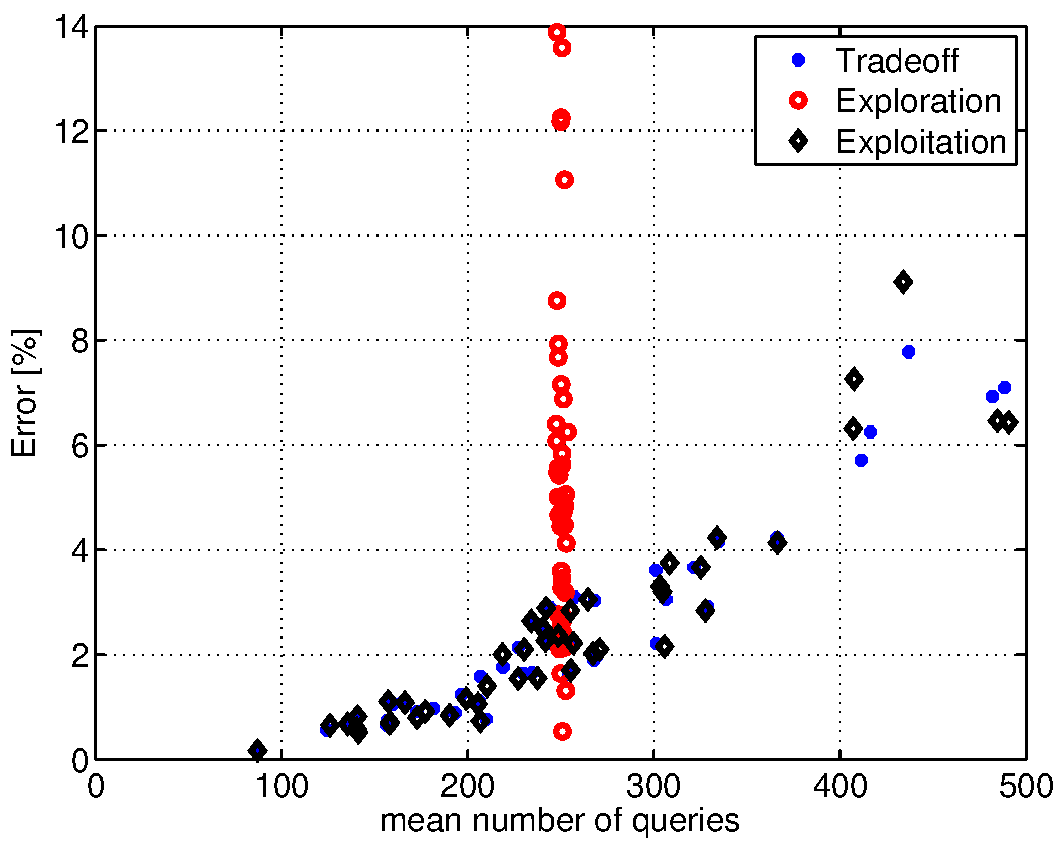
\includegraphics[width=0.27\textwidth]{figs/mnist2b-eps-converted-to.png}\label{fig:mnist2}}
%\caption{Left: mean of fraction no. of mistakes SHAMPO made during training time on MNIST of all examples and only queried. Right: test error vs no. of queries is plotted for all MNIST one-vs-one problems.}
%\end{centering}
%%\vspace{-0.3cm}
%\end{wrapfigure}

\begin{figure}[!t]
\begin{centering}
\subfigure[MNIST one-vs-one]{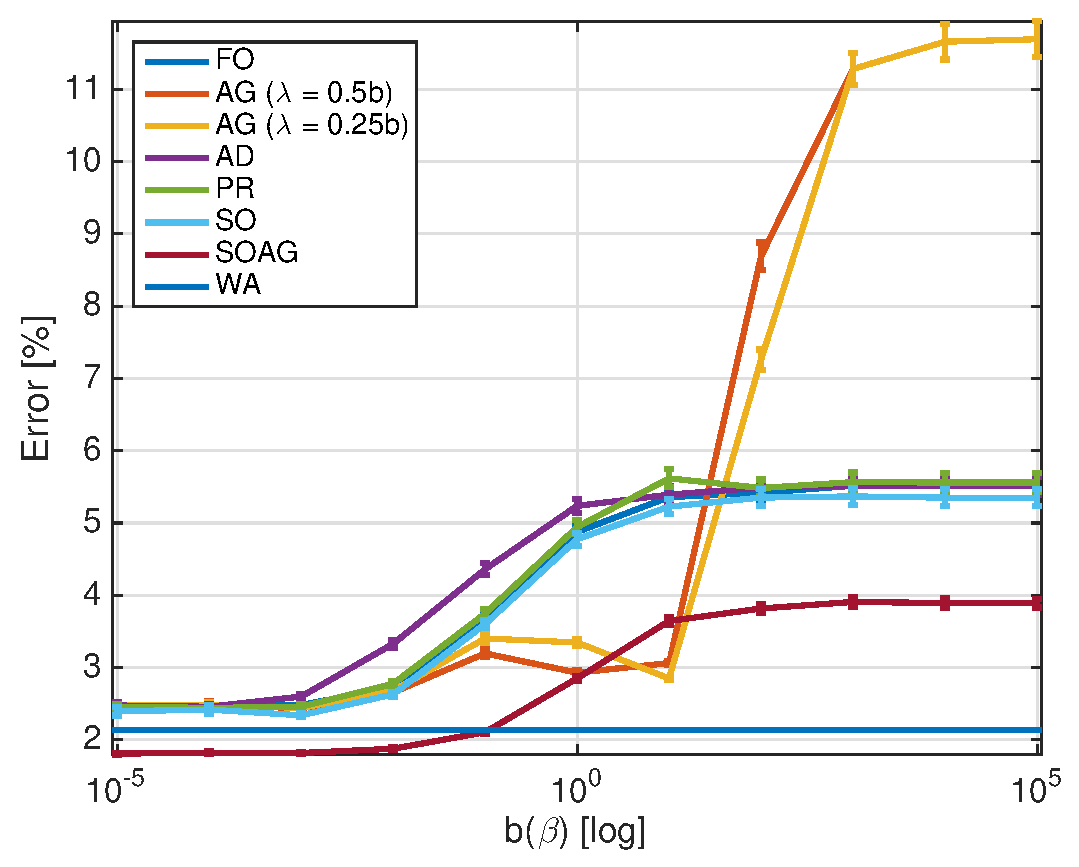
\includegraphics[width=0.4\textwidth]{figs/test-m1.eps}\label{fig:bars1}}
\subfigure[MNIST one-vs-rest]{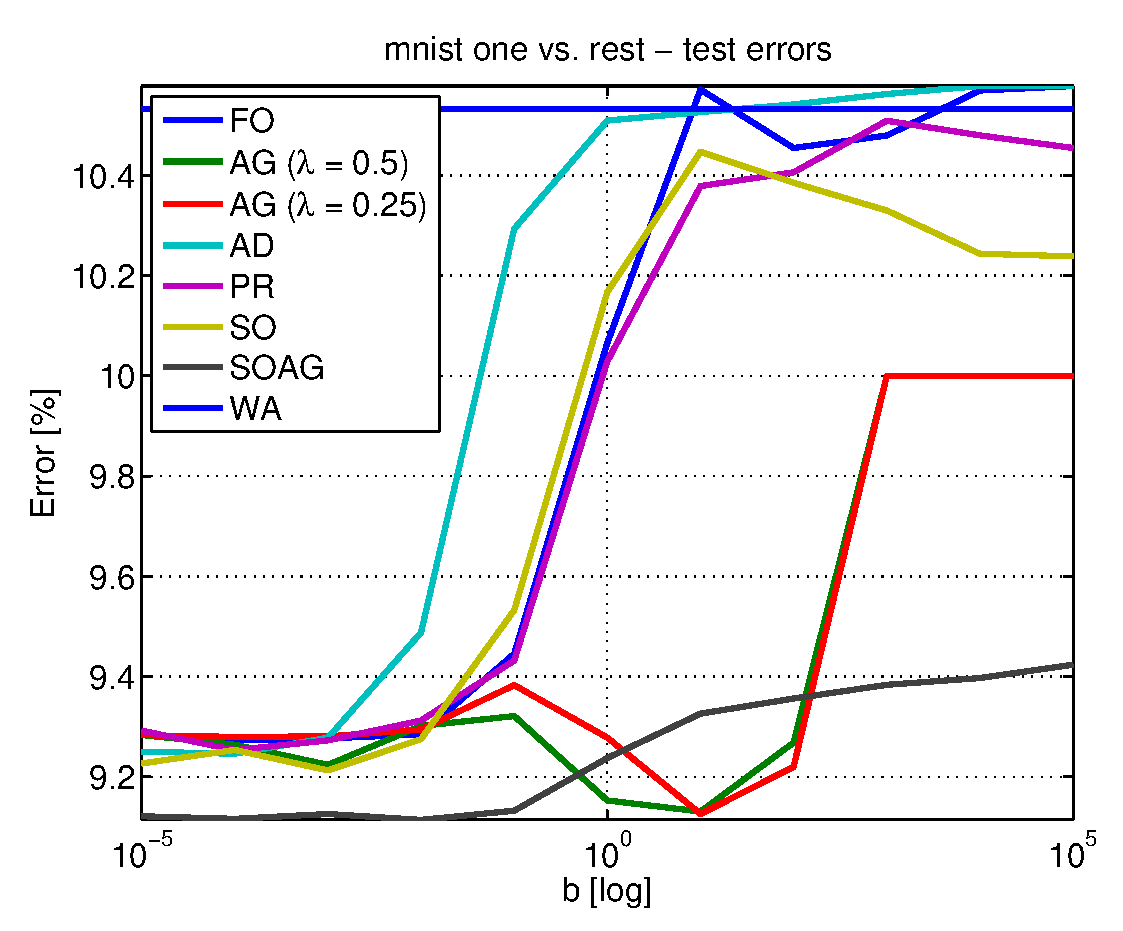
\includegraphics[width=0.4\textwidth]{figs/test-mr.eps}\label{fig:bars2}}
\subfigure[USPS one-vs-one]{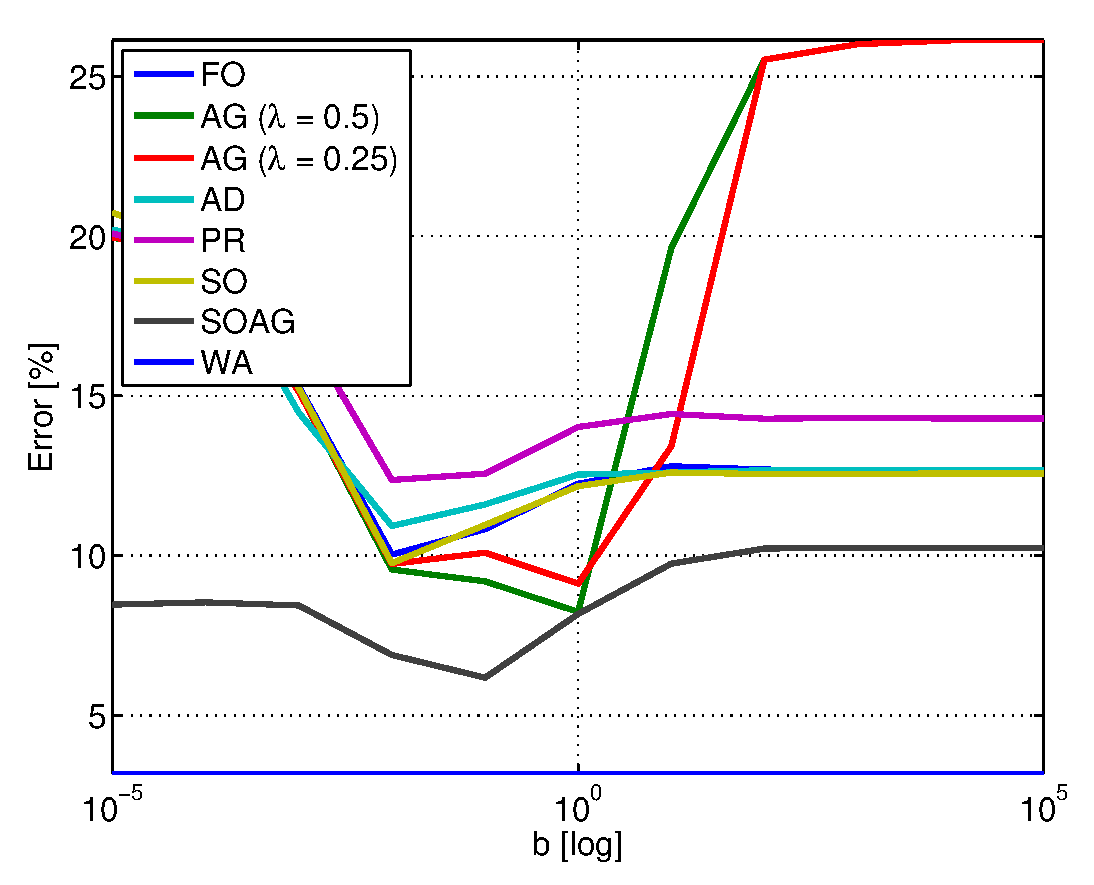
\includegraphics[width=0.4\textwidth]{figs/test-u1.eps}\label{fig:bars1}}
\subfigure[USPS one-vs-rest]{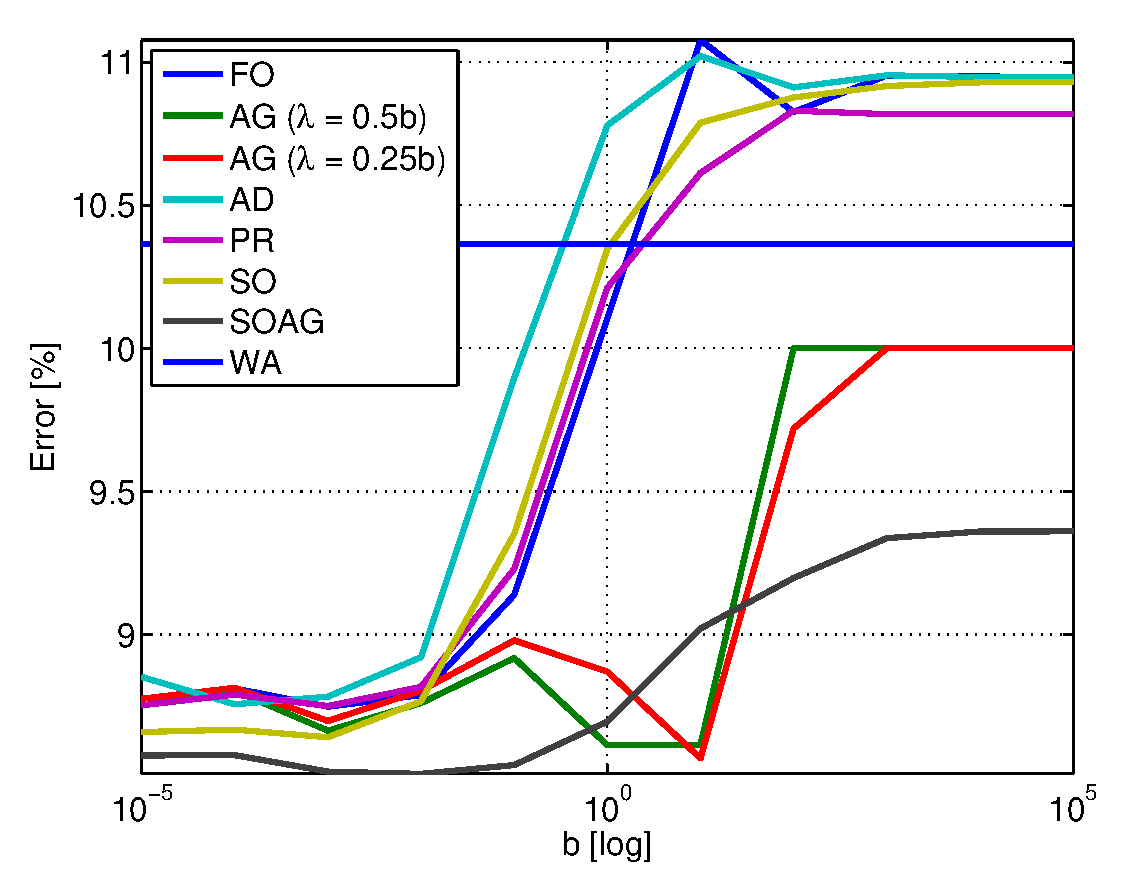
\includegraphics[width=0.4\textwidth]{figs/test-ur.eps}\label{fig:bars2}}
\subfigure[VJ one-vs-one]{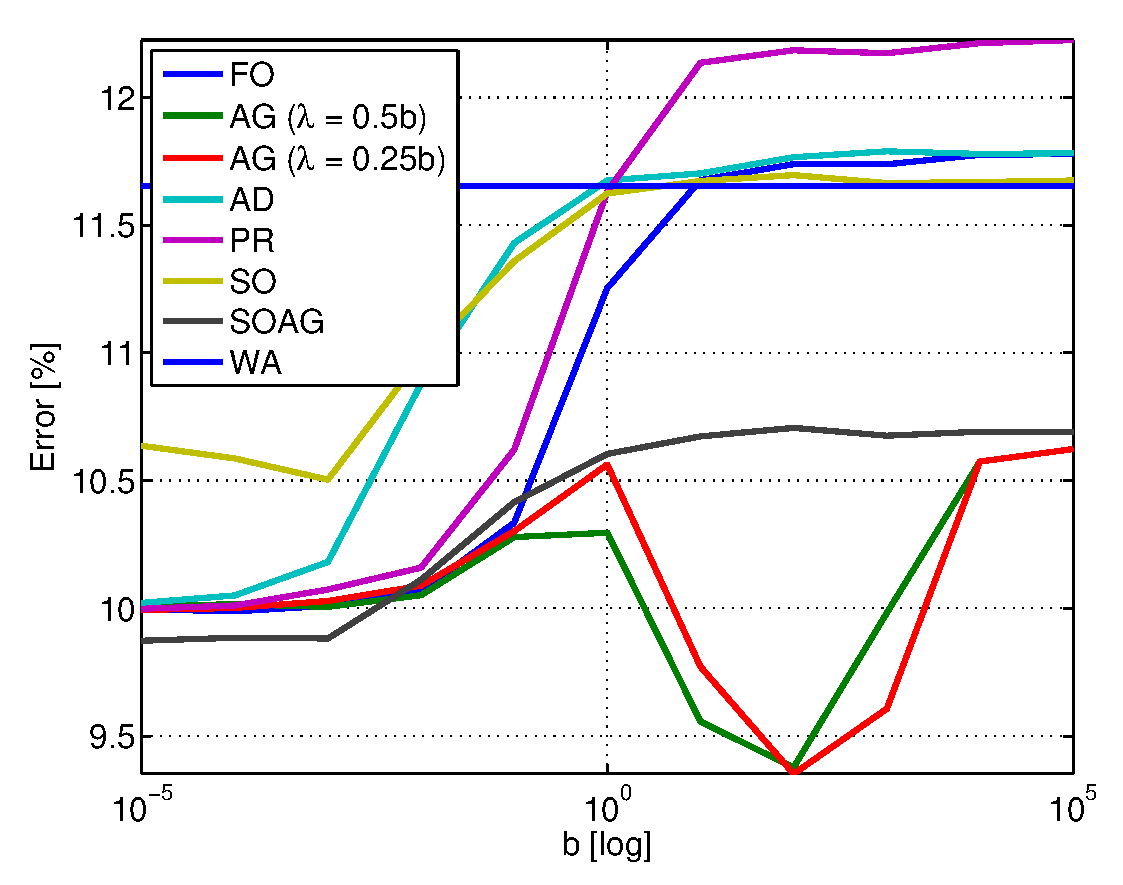
\includegraphics[width=0.4\textwidth]{figs/test-v1.eps}\label{fig:bars1}}
\subfigure[VJ one-vs-rest]{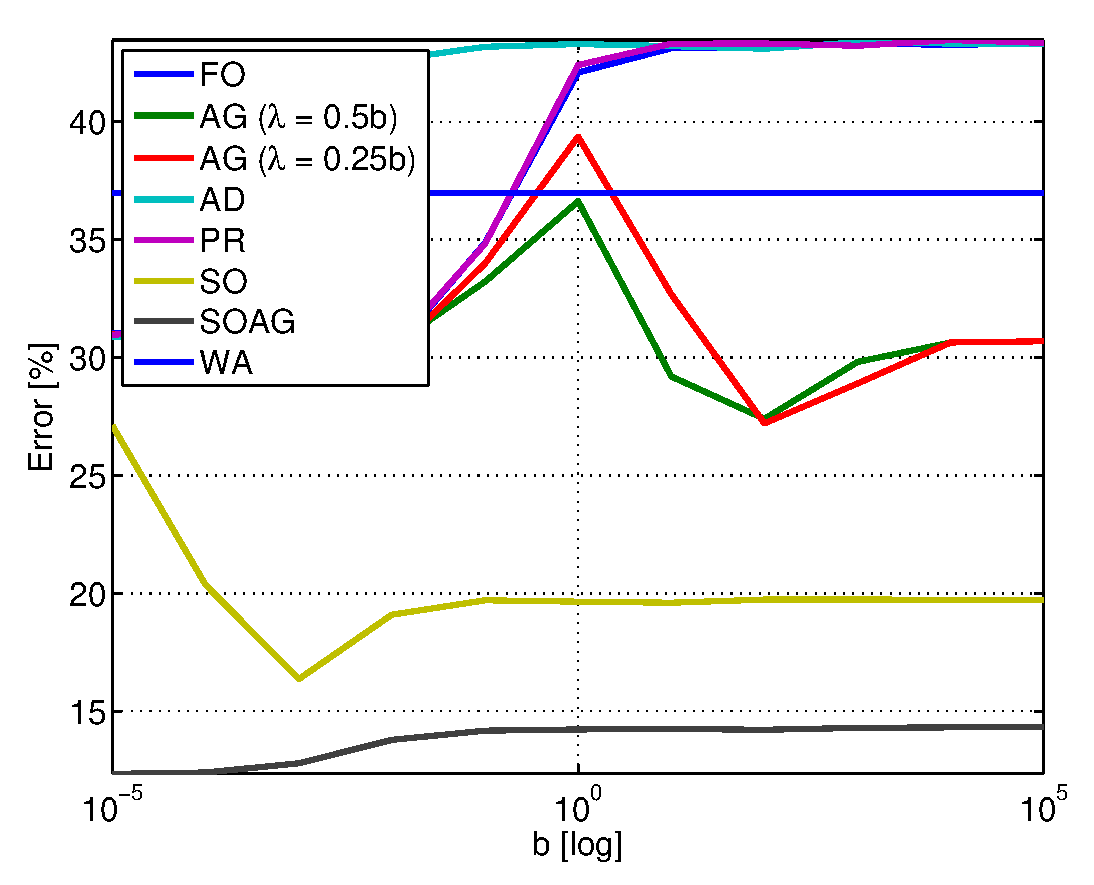
\includegraphics[width=0.4\textwidth]{figs/test-vr.eps}\label{fig:bars2}}
\subfigure[NLP ove-vs-one]{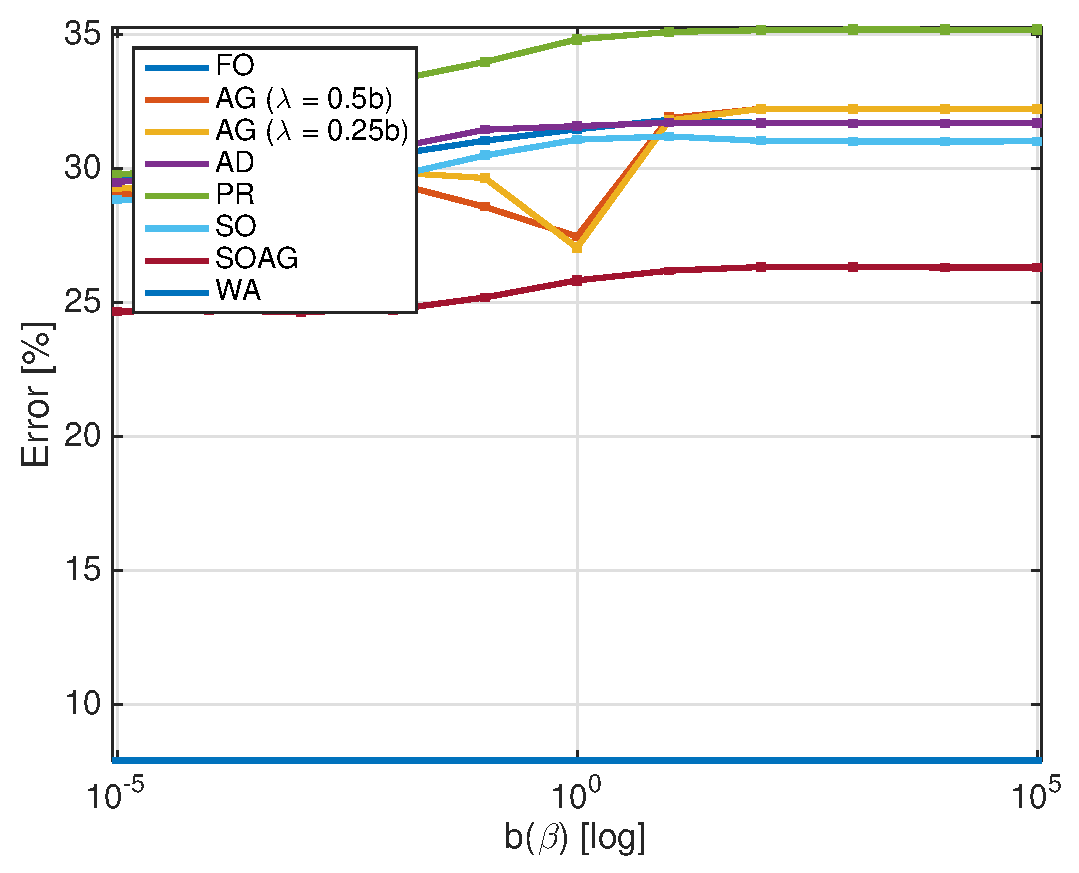
\includegraphics[width=0.4\textwidth]{figs/test-n.eps}\label{fig:bars2}}
\caption{test error}
\end{centering}
\vspace{-0.5cm}
\end{figure}

\begin{figure}[!t]
\begin{centering}
\subfigure[MNIST one-vs-one]{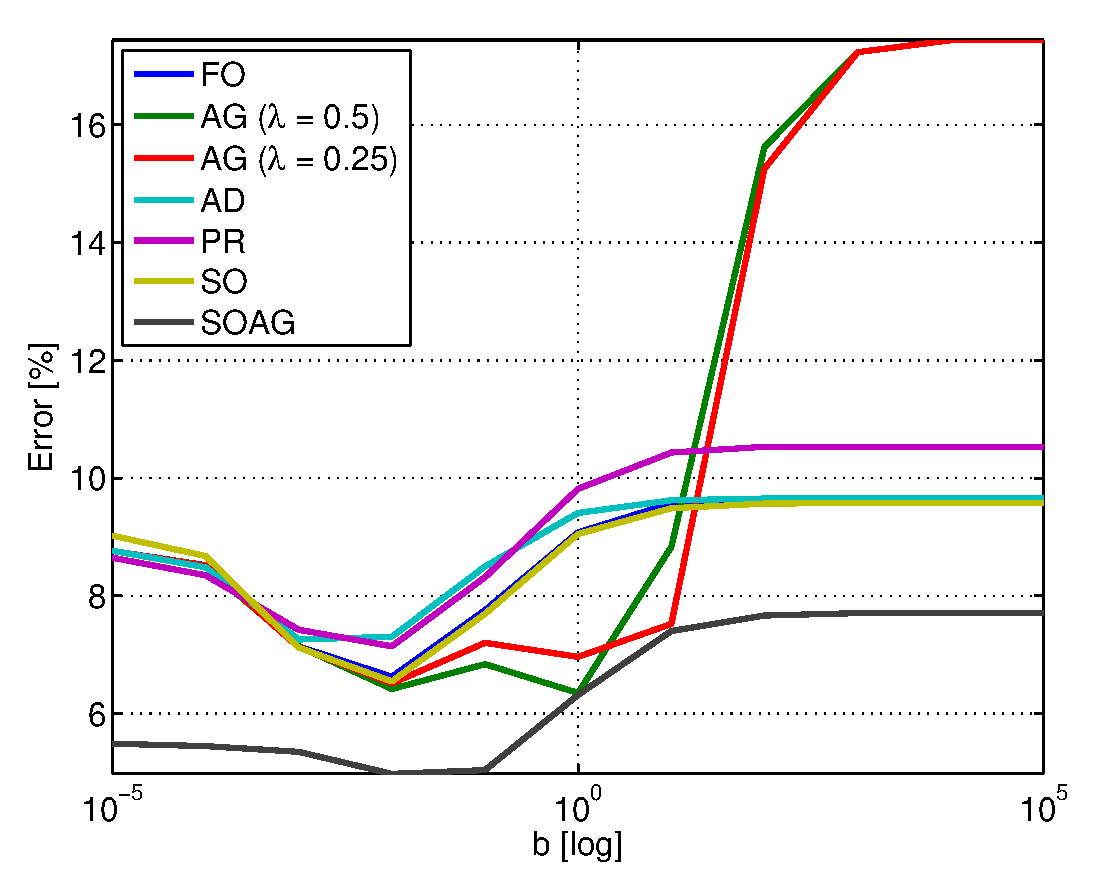
\includegraphics[width=0.4\textwidth]{figs/train-m1.eps}\label{fig:bars1}}
\subfigure[MNIST one-vs-rest]{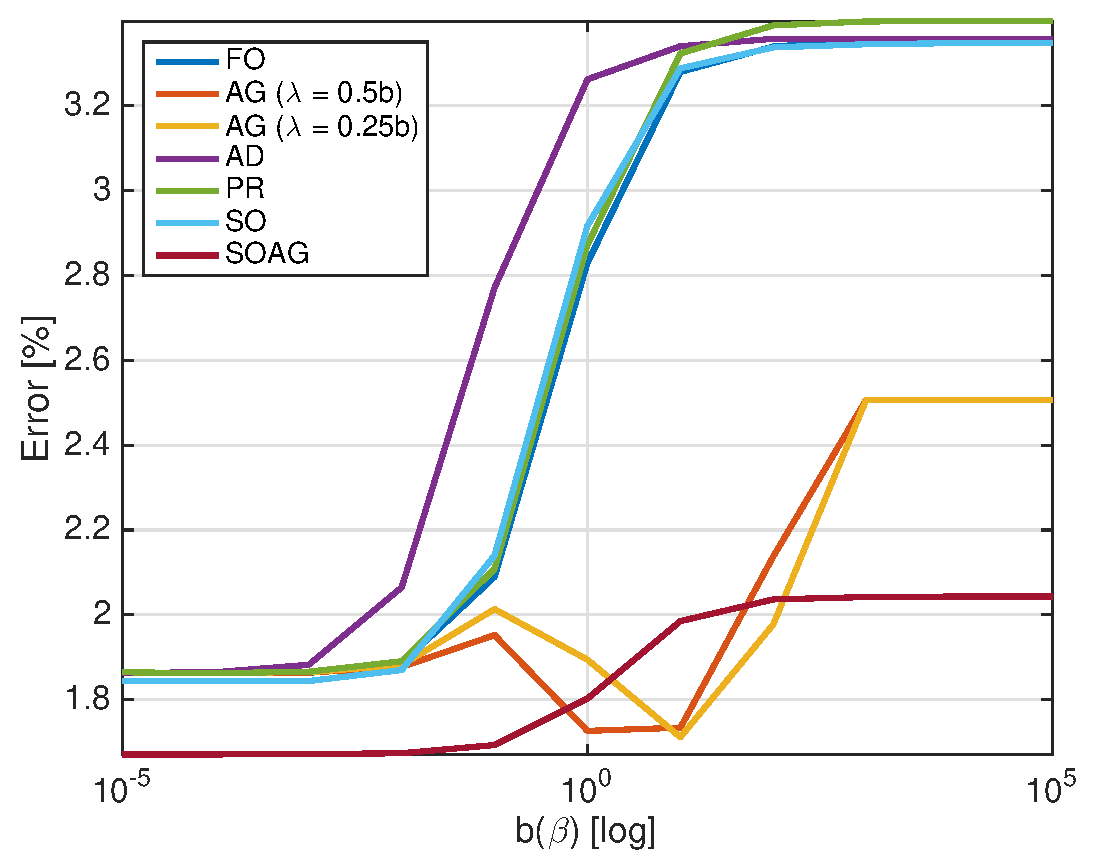
\includegraphics[width=0.4\textwidth]{figs/train-mr.eps}\label{fig:bars2}}
\subfigure[USPS one-vs-one]{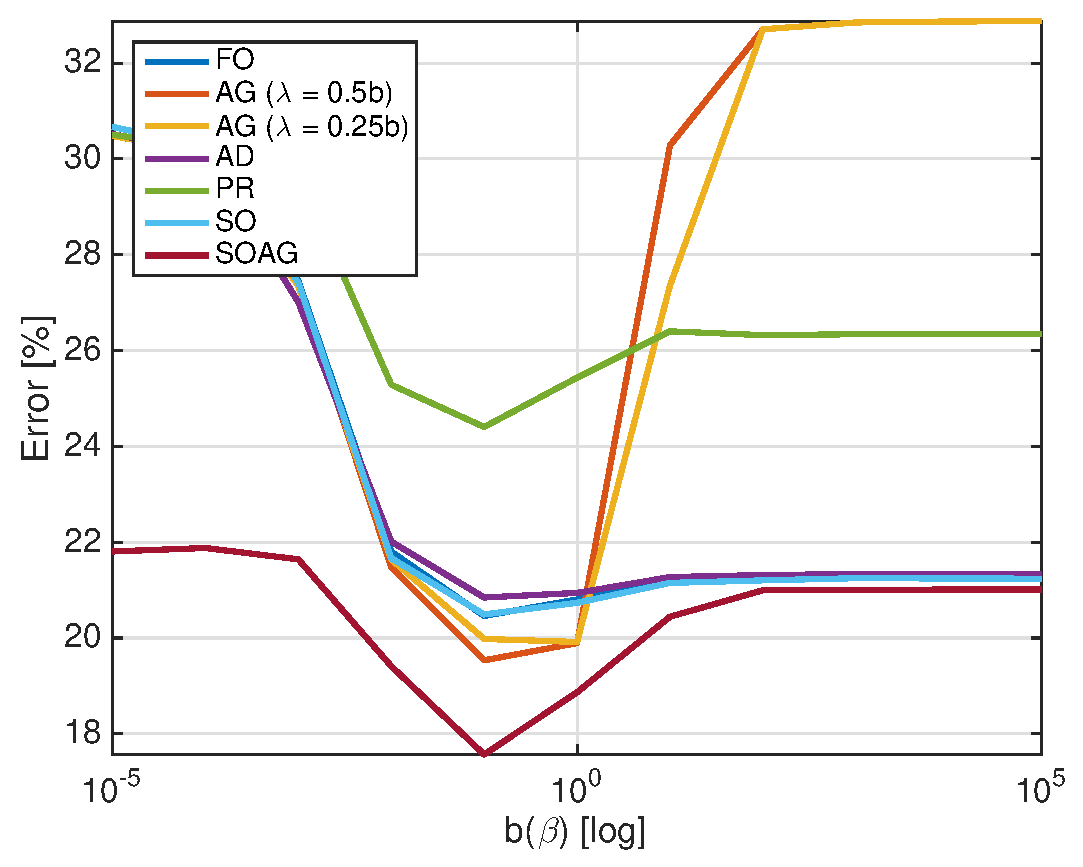
\includegraphics[width=0.4\textwidth]{figs/train-u1.eps}\label{fig:bars1}}
\subfigure[USPS one-vs-rest]{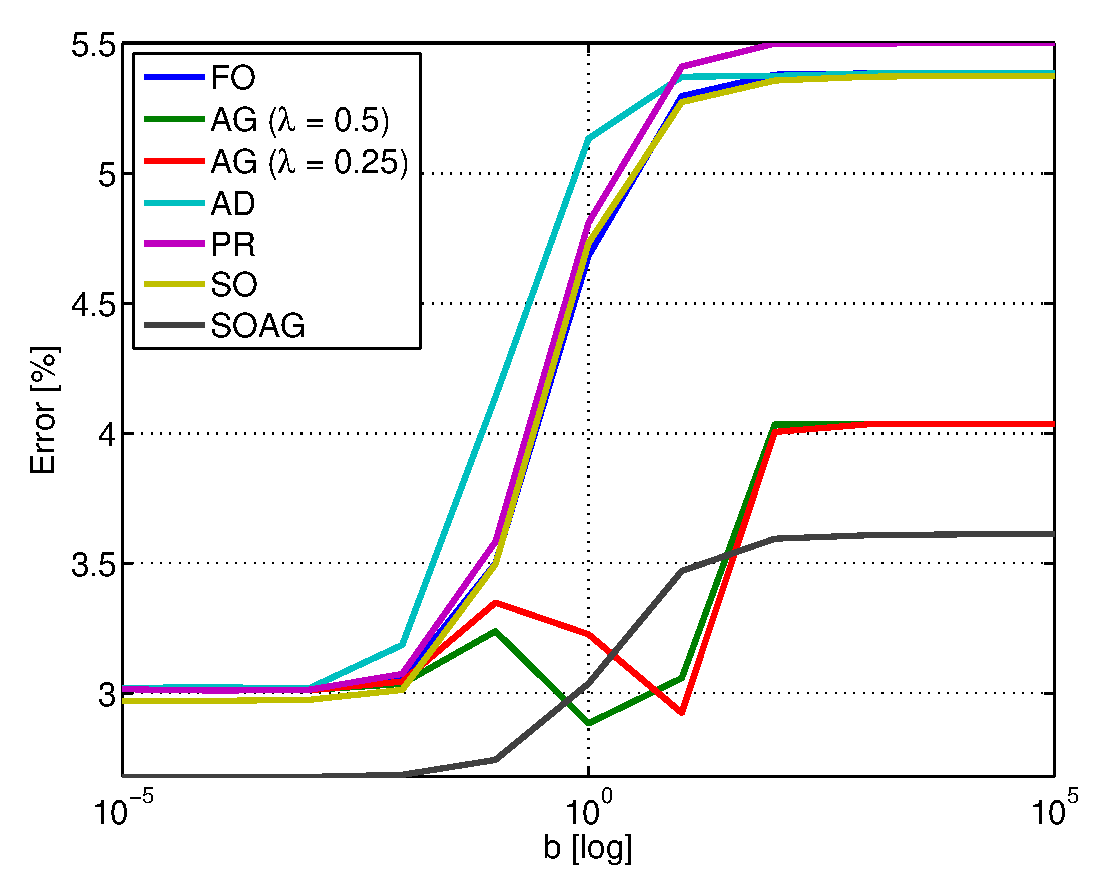
\includegraphics[width=0.4\textwidth]{figs/train-ur.eps}\label{fig:bars2}}
\subfigure[VJ one-vs-one]{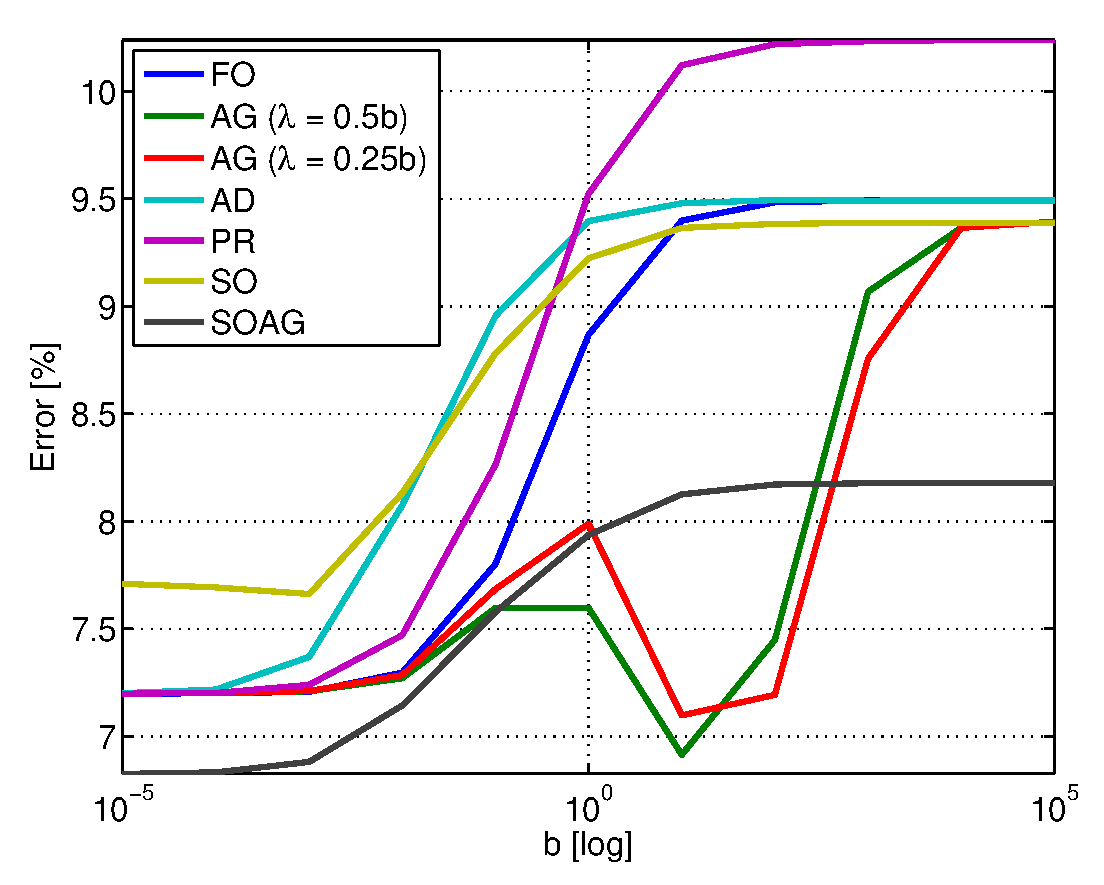
\includegraphics[width=0.4\textwidth]{figs/train-v1.eps}\label{fig:bars1}}
\subfigure[VJ one-vs-rest]{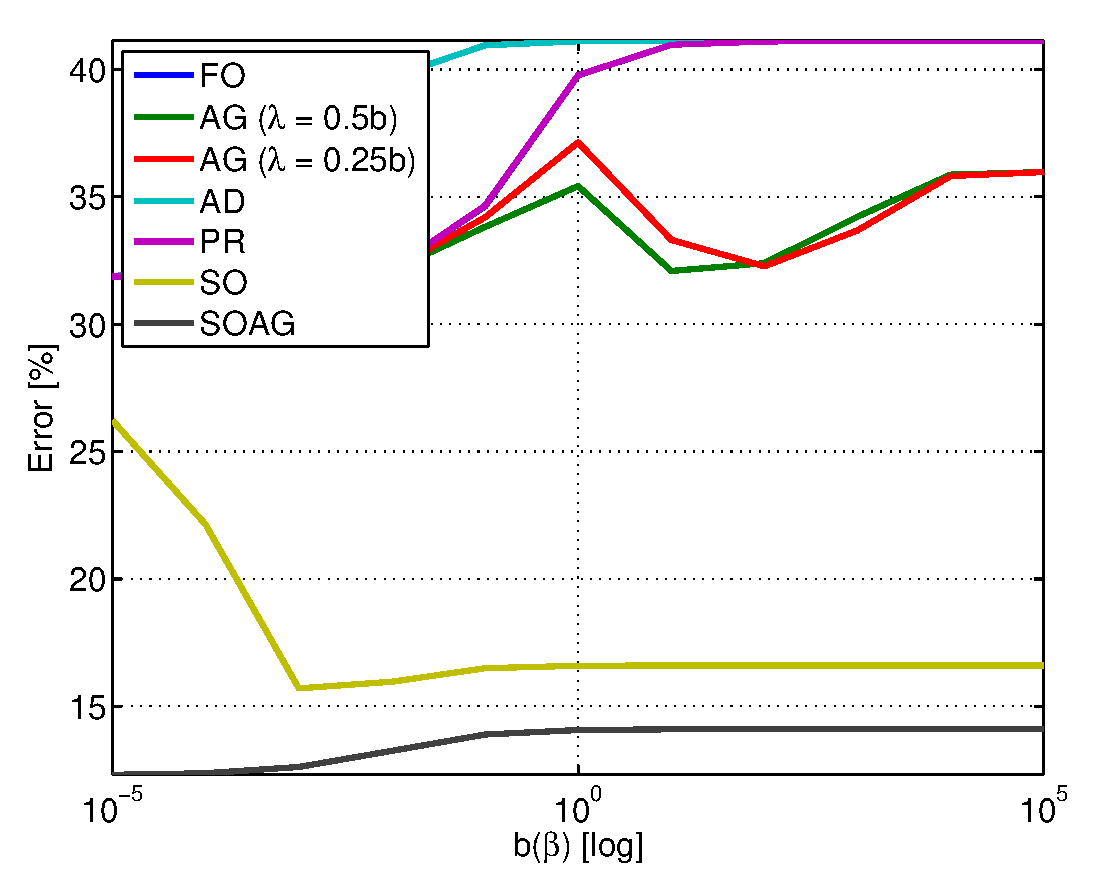
\includegraphics[width=0.4\textwidth]{figs/train-vr.eps}\label{fig:bars2}}
\subfigure[NLP one-vs-one]{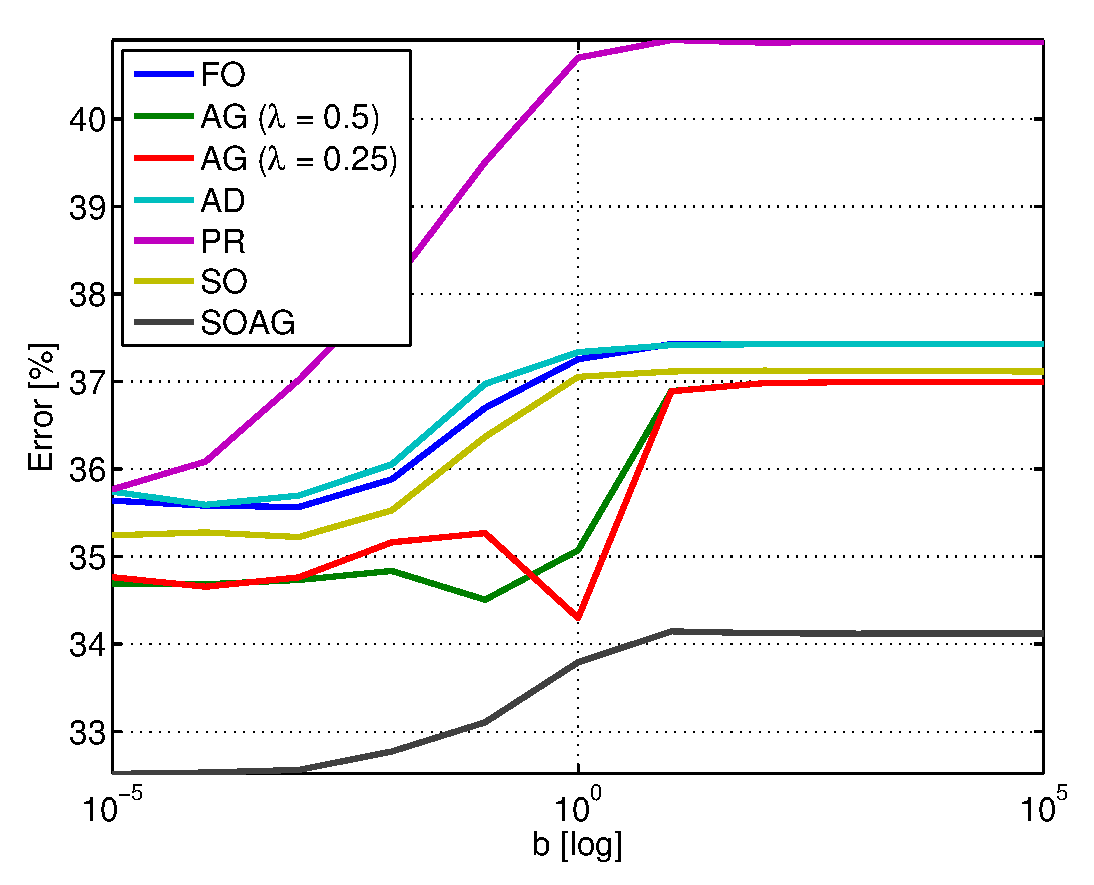
\includegraphics[width=0.4\textwidth]{figs/train-n.eps}\label{fig:bars2}}
\caption{train }
\end{centering}
\vspace{-0.5cm}
\end{figure}

\begin{figure}[!t]
\begin{centering}
\subfigure[MNIST one-vs-one]{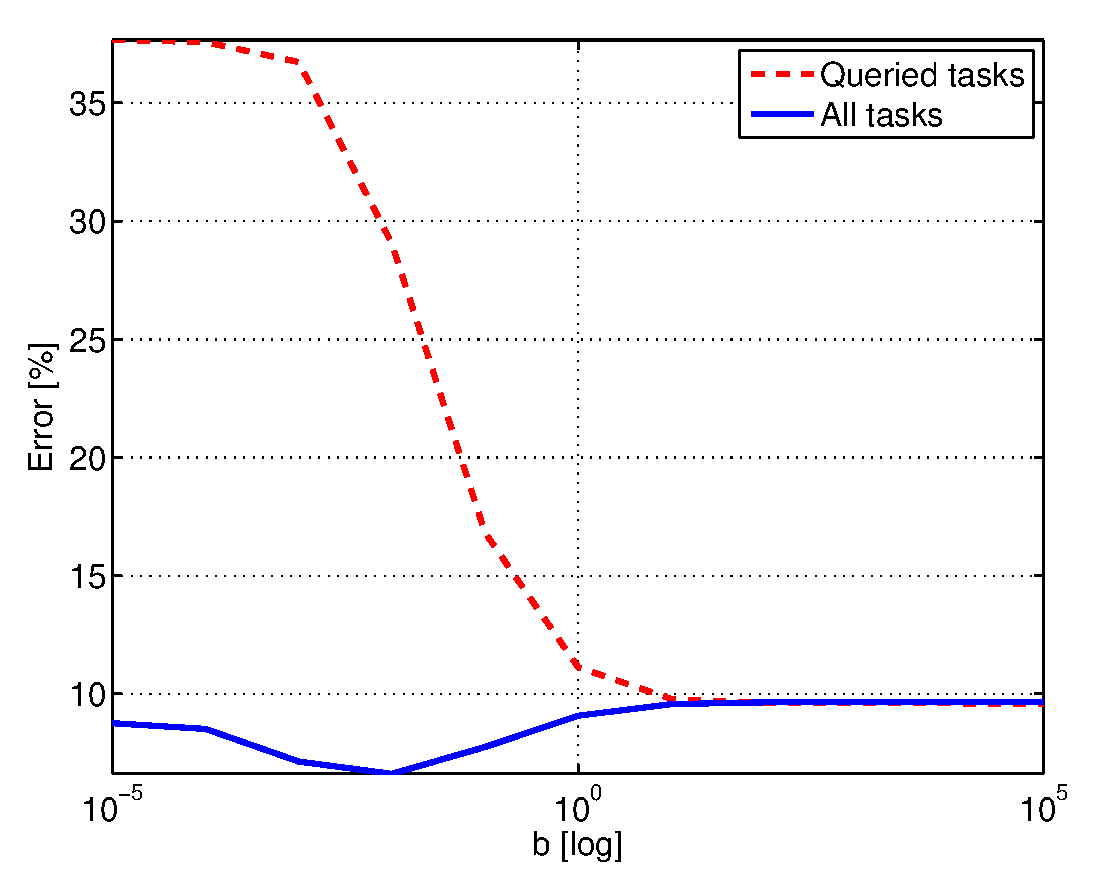
\includegraphics[width=0.4\textwidth]{figs/queried-m1.eps}\label{fig:bars1}}
\subfigure[MNIST one-vs-rest]{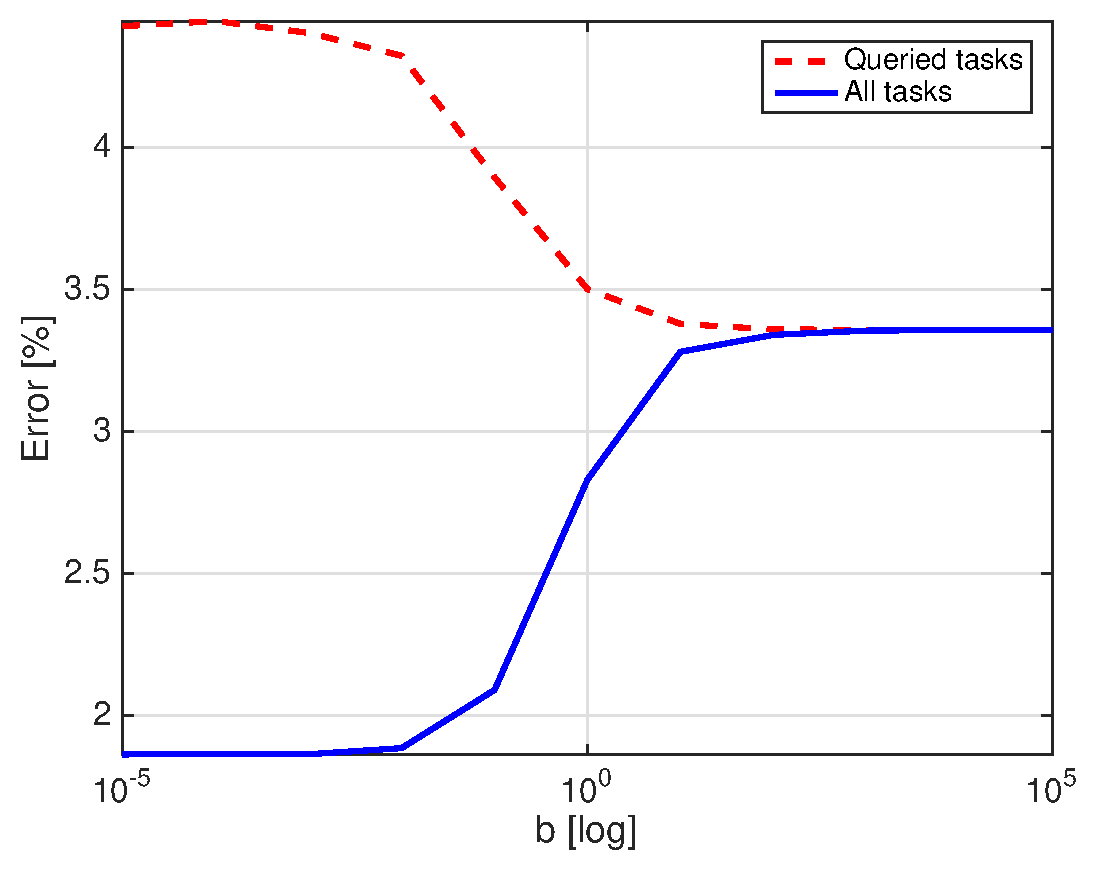
\includegraphics[width=0.4\textwidth]{figs/queried-mr.eps}\label{fig:bars2}}
\subfigure[USPS one-vs-one]{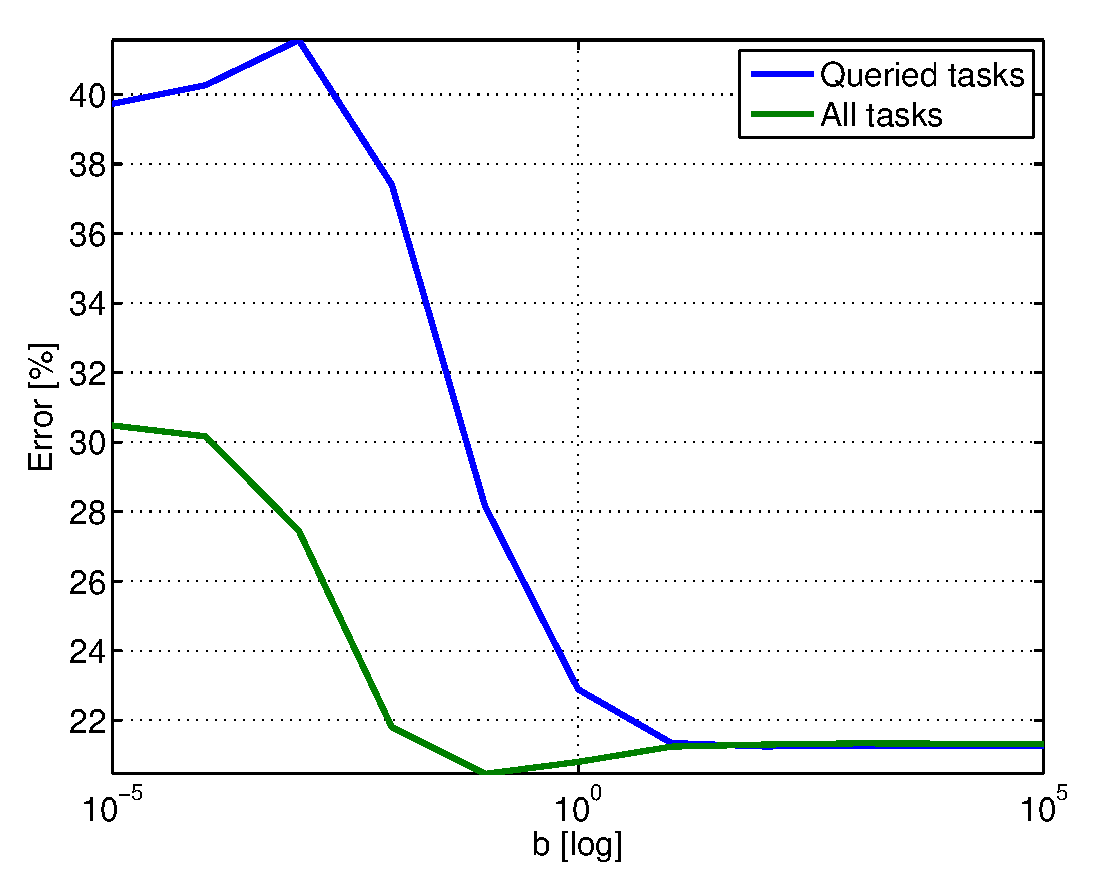
\includegraphics[width=0.4\textwidth]{figs/queried-u1.eps}\label{fig:bars1}}
\subfigure[USPS one-vs-rest]{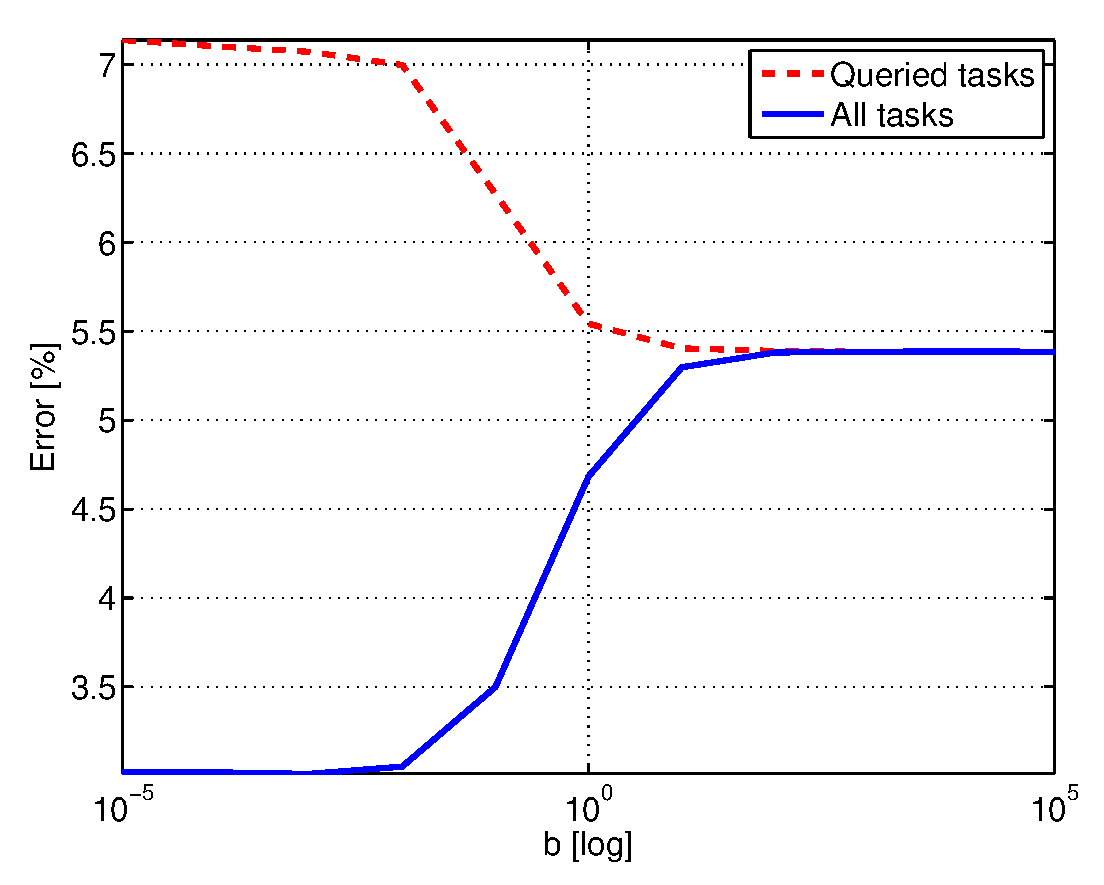
\includegraphics[width=0.4\textwidth]{figs/queried-ur.eps}\label{fig:bars2}}
\subfigure[VJ one-vs-one]{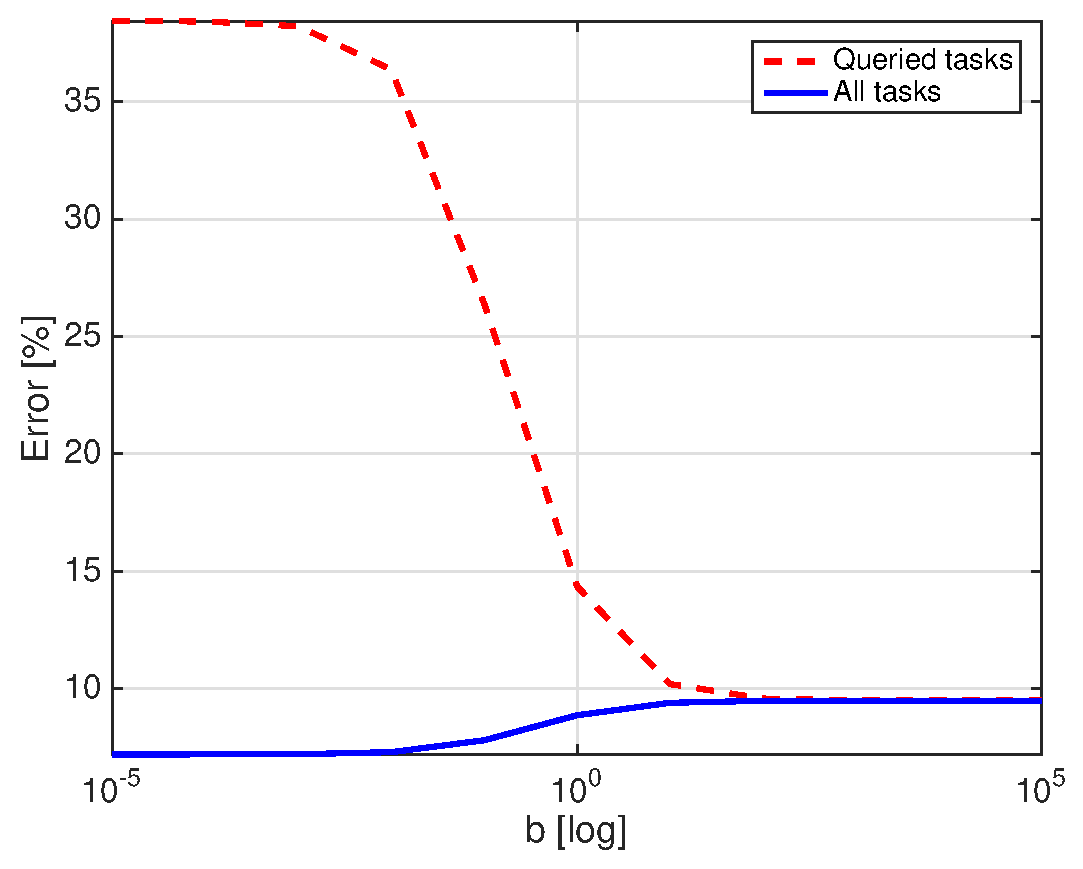
\includegraphics[width=0.4\textwidth]{figs/queried-v1.eps}\label{fig:bars1}}
\subfigure[VJ one-vs-rest]{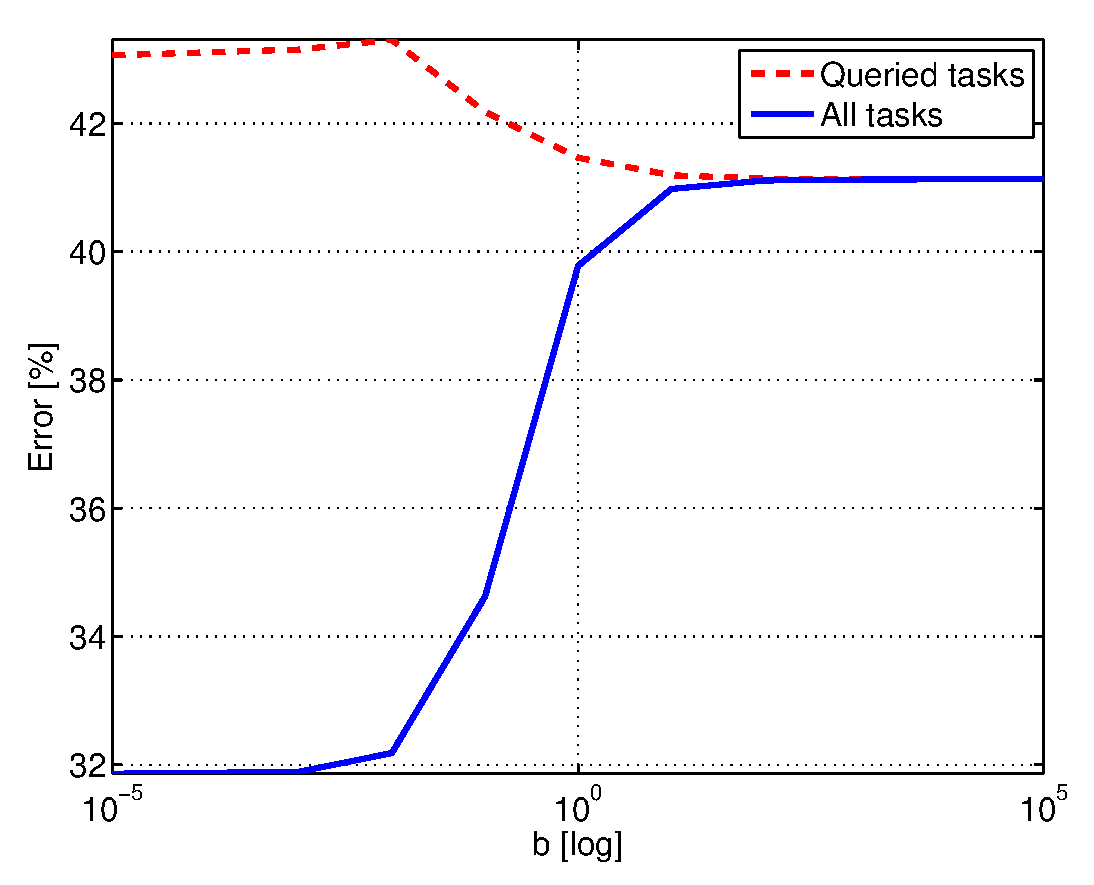
\includegraphics[width=0.4\textwidth]{figs/queried-vr.eps}\label{fig:bars2}}
\subfigure[NLP one-vs-one]{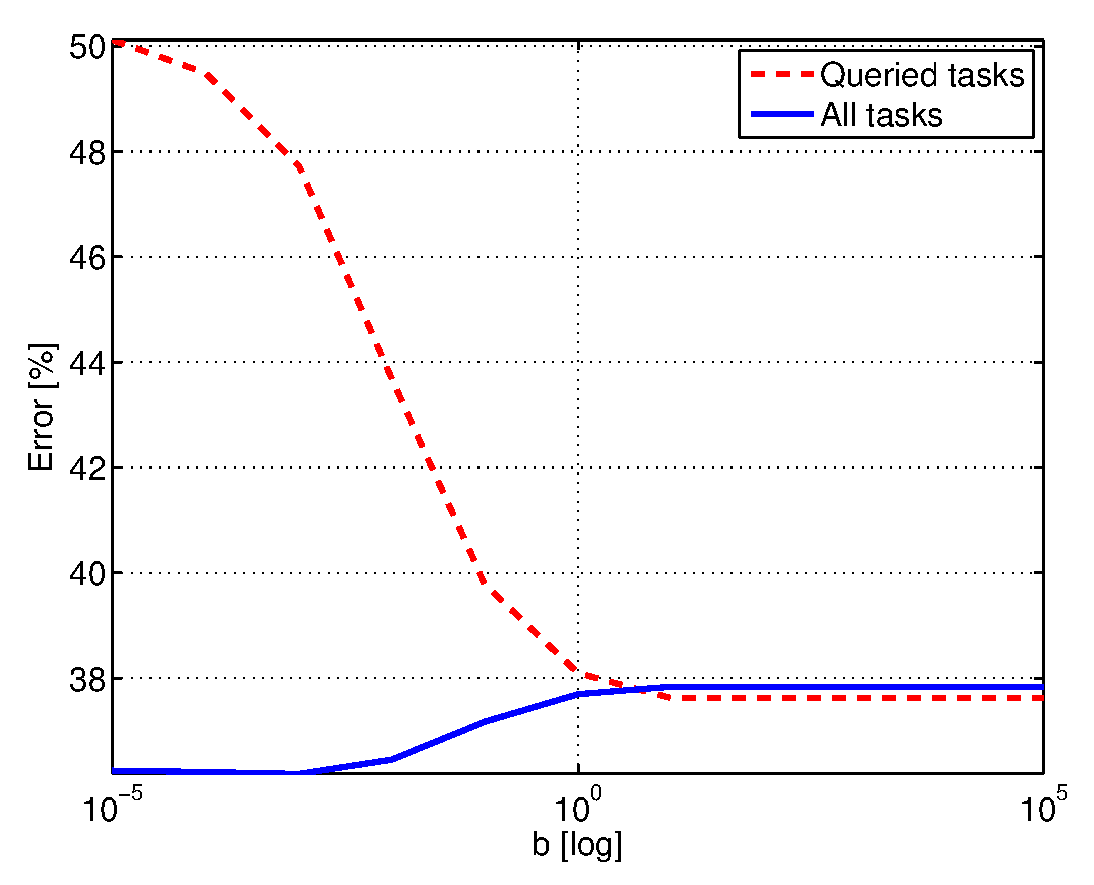
\includegraphics[width=0.4\textwidth]{figs/queried-n.eps}\label{fig:bars2}}
\caption{train error queried vs all -FO algorithm}
\end{centering}
\vspace{-0.5cm}
\end{figure}

We evaluated the SHAMPO algorithm using four datasets: USPS, MNIST (both OCR), Vocal Joystick 
(VJ, vowel recognition) and document classification. 
The USPS dataset, contains $7,291$ training examples and $2,007$ test examples, each one of them is a 
$16\times16$ pixels gray-scale images converted to a $256$ dimensional vector. 
The MNIST dataset with $28\times28$ gray-scale images, contains $60,000$ 
examples in the training set and $10,000$ in the testing set. and  In both cases there are $10$ possible labels, digits. The VJ tasks is to predict a vowel from 
eight possible vowels. Each example is a frame of spoken value described with $13$ MFCC coefficients 
transformed into 27 features. There are $572,911$ training examples and $236,680$ test examples. 
We created binary tasks from these multi-class datasets using two reductions: One-vs-Rest setting and 
One-vs-One setting. For example, in both USPS and MNIST there are $10$ binary one-vs-rest tasks and 
$45$ binary one-vs-one tasks.  The NLP document classification include of spam filtering, news items and 
news-group classification, sentiment classification, and product domain categorization. 
A total of $31$ binary prediction tasks over all, with a total of $252,609$ examples, and input dimension 
varying between $8,768$ and $1,447,866$. Details of the individual binary tasks can be found 
elsewhere~\cite{Crammer:2012:CLC:2343676.2343704}.
This yielded seven collections (USPS, MNIST and VJ; each as one-vs-rest or one-vs-one) and document 
classification.

We evaluated two baselines as well as our algorithm. Algorithm {\em uniform} picks a random task to be 
queried and updated (corresponding to $b\rightarrow\infty$), {\em exploit} which picks the tasks with the 
lowest absolute margin (i.e. the ``hardest instance''), this combination corresponds to $b \approx 0$ of 
SHAMPO. We tried for SHAMPO $13$ values for $b$, equally spaced on a logarithmic scale. 
All algorithms made a single pass over the training data.  We ran two version of the algorithm: 
plain version, without aggressiveness (updates on mistakes only, $\lambda=0$) and an 
Aggressive version $\lambda=b/2$ (we tried lower values of $\lambda$ as in the bound, 
but we found that $\lambda=b/2$ gives best results), both with uniform prior ($a_i=1$). 
We used separate training set and a test set, to build a model and evaluate it.
%Each algorithm was trained on a training set and evaluated on a test set.

Results are evaluated using $2$ quantities. First, the average test error (over all the dataset combinations) 
and the average score. For each combination we assigned a score of $1$ to the algorithm with the lowest 
test error, and a score of $2$, to the second best, and all the way up to a score of $6$ to the algorithm with 
the highest test error.
%
%For each one of those algorithms we compared three variations: \textit{exploration} ($b\rightarrow 0$), \textit{uniform} distribution ($b\rightarrow \infty$) and \textit{our} method (we found $b=1$ to be a good value in our setting).
\vspace{-0.1cm}
\paragraph{Multi-task Binary Classification :}
\figref{fig:bars1} and \figref{fig:bars2} show the test error of the three algorithms on two of document 
classification combinations, with four and eight tasks. Clearly, not only SHAMPO performs better, 
but it does so on each task individually. (Our analysis above bounds the total number of mistakes over all 
tasks.) \figref{fig:test_error} shows the average test error vs $b$ using the one-vs-one binary USPS 
problems for the three variants of SHAMPO: non-aggressive (called plain), aggressive and aggressive with 
prior.Clearly, the plain version does worse than both the aggressive version and the non-uniform prior version. 
For other combinations %(e.g. document classification)
the prior was not always improving results. We hypothesise that this is because our heuristic may 
yield a bad prior which is not focusing the algorithm on the right (hard) tasks. 


\begin{table}[t]\label{tab:table1}
\begin{centering}
\caption{Test errors percentage . Scores are shown in parenthesis.}
{\small
\begin{tabular}{|l|r|r|r|r|r|r|}
\hline
                         & \multicolumn{3}{c|}{\textbf{Aggressive $\lambda=b/2$}}               & \multicolumn{3}{c|}{\textbf{Plain}}                 \\ \hline
\textit{Dataset}         & \textit{exploit} & \textit{SHAMPO}         & \textit{uniform} & \textit{exploit} & \textit{SHAMPO} & \textit{uniform} \\ \hline
{VJ 1 vs 1 }        & 5.22 (2.9)       & \textbf{4.57 (1.1)}   & 5.67 (3.9)       & 5.21 (2.7)       & 6.93 (4.6)    & 6.26 (5.8)       \\
\textrm{VJ 1 vs Rest}    & 13.26 (3.5)      & \textbf{11.73 (1.2)} & 12.43 (2.5)      & 13.11 (3.0)        & 14.17 (5.0)     & 14.71 (5.8)     \\
\textrm{USPS 1 vs 1}      & 3.31 (2.5)       & \textbf{2.73 (1.0)}     & 19.29 (6.0)        & 3.37 (2.5)       & 4.83 (4.0)      & 5.33 (5,0)         \\
\textrm{USPS 1 vs Rest}  & 5.45 (2.8)      & \textbf{4.93 (1.2)}  & 10.12 (6.0)        & 5.31 (2.0)         & 6.51 (4.0)      & 7.06 (5.0)         \\
\textrm{MNIST 1 vs 1}     & 1.08 (2.3)       & \textbf{0.75 (1.0)}     & 5.9 (6.0)         & 1.2 (2.7)       & 1.69 (4.1)      & 1.94 (4.9)     \\
\textrm{MNIST 1 vs Rest} & 4.74 (2.8)      & \textbf{3.88 (1.0)}     & 10.01 (6.0)       & 4.44 (2.8)      & 5.4 (3.8)    & 6.1 (5.0)          \\
\textrm{NLP documents} & 19.43 (2.3)     & \textbf{16.5 (1.0)}     & 23.21 (5.0)        & 19.46 (2.7)     & 21.54 (4.7)  & 21.74 (5.3)     \\
\textrm{MIXED}           & 2.75 (2.4)       & \textbf{2.06 (1.0)}     & 13.59 (6.0)        & 2.78 (2.6)       & 4.2 (4.3)     & 4.45 (4.7)       \\ \hline
\textit{Mean score}      & (2.7)           & \textbf{(1.1)}       & (5.2)           & (2.6)           & (4.3)        & (5.2)           \\ \hline
\end{tabular}
}
\end{centering}
\vspace{-0.5cm}
\end{table}
Results  are summarized in Tab.~1. In general {\em exploit} is better than {\em uniform} and aggressive 
is better than non-aggressive. Aggressive SHAMPO yields the best results both evaluated as average 
(over tasks per combination and over combinations). Remarkably, even in the mixed dataset 
(where tasks are of different nature: images, audio and documents), the aggressive SHAPO improves over 
uniform (4.45\% error) and the aggressive-exploit baseline (2.75\%), and achieves a test error of 2.06\%.
% \begin{table}[!t]\label{tab:table2}
% \caption{Test errors percentage. The scores are shown in the parenthesis.}
% \begin{center}
% {\small
% \begin{tabular}{|l|r|r|r|r|r|r|}
% \hline
%                         & \multicolumn{3}{c|}{\textbf{Aggressive $\lambda$=b}}           & \multicolumn{3}{c|}{\textbf{Aggressive $\lambda$=b with prior}}  \\ \hline
% \textit{Dataset}        & \textit{exploit} & \textit{ours}     & \textit{uniform} & \textit{exploit} & \textit{ours}        & \textit{uniform} \\ \hline
% {USPS 1 vs 1}     & 3.31 (3.9)       & 2.73 (2.9)        & 19.29 (5.6)      & 1.92 (2.2)       & \textbf{1.47 (1.0)}    & 17.66 (5.4)      \\
% {USPS 1 vs Rest} & 5.45 (3.5)       & \textbf{4.93 }(2.0) & 10.12 (5.7)     & 5.23 (2.8)      & 4.97 \textbf{(1.7)} & 9.64 (5.3)      \\ \hline
% \end{tabular}
% }
% \end{center}
% \end{table}

Next, we focus on the problems that the algorithm chooses to annotate on each iteration for various values 
of $b$. \figref{fig:mnist1} shows the total number of mistakes SHAMPO made during training time on MNIST, 
we show two quantities: fraction of mistakes over all training examples (denoted by ``total'' - blue) 
and fraction of mistakes over only queried examples (denoted by ``queried'' - dashed red). 
In pure exploration (large %values of
$b$) both quantities are the same, as the choice of problem to be labeled is independent of the problem and 
example, and essentially the fraction of mistakes in queried examples is a good estimate of the fraction of 
mistakes over all examples. The other extreme is when performing pure exploitation (low %values of
$b$), here the fraction of mistakes made on queried examples went up, while the overall fraction of mistakes 
went down. This indicates that the algorithm indeed focuses its queries on the harder inputs, which in turn, 
improves overall training mistake. There is a sweet point $b\approx 0.01$ for which SHAMPO is still 
focusing on the harder examples, yet reduces the total fraction of training mistakes even more. 
The existence of such tradeoff is predicted by \thmref{thm:bound}. % Finally, note that in all cases, the value 
of $b$ which minimizes the mean test error, is about the point for which there is a change in the error of 
queried examples (the only quantity SHAMPO observes), which provides a rough rule-of-thumb to pick 
$b$ automatically on-the-fly.


Another perspective of the phenomena is that for values of $b\ll \infty$ SHAMPO focuses on the harder 
examples, is illustrated in \figref{fig:mnist2} where test error vs number of queries is plotted for each 
problem for MNIST. We show three cases: uniform, exploit and a mid-value of $b\approx 0.01$ which 
tradeoffs exploration and exploitation. Few comments: First, when performing uniform querying, all 
problems have about the same number of queries ($266$), close to the number of examples per problem 
($12,000$), divided by the number of problems ($45$). Second, when having a tradeoff between exploration 
and exploitation, harder problems (as indicated by test error) get more queries than easier problems. 
For example, the four problems with test error greater than $6\%$ get at least $400$ queries, which is 
about twice the number of queries received by each of the $12$ problems with test error less than $1\%$. 
Third, as a consequence, SHAMPO performs equalization, giving the harder problems more labeled data, 
and as a consequence, reduces the error of these problems, however, is not increasing the error of the 
easier problems which gets less queries (in fact it reduces the test error of all 45 problems!). 
The tradeoff mechanism of SHAMPO, reduces the test error of each problem by more than $40\%$ 
compared to full exploration. Fourth, exploits performs similar equalization, yet in some hard tasks it 
performs worse than SHAMPO. This could be because it overfits the training data, by focusing on 
hard-examples too much, as SHAMPO has a randomness mechanism.


Indeed, Table~1 shows that aggressive SHAMPO outperforms better alternatives. Yet, we claim that a 
good prior may improve results. We compute prior over the 45 USPS tasks, by running the perceptron 
algorithm on $1000$ examples and computing the number of mistakes.  
We set the prior to be proportional to this number. We then reran aggressive SHAMPO with prior, 
comparing it to aggressive SHAMPO with no prior (i.e. $a_i=1$). 
Aggressive SHAMO with prior achieves average error of $1.47$ (vs. $2.73$ with no prior) on 1-vs-1 USPS 
and $4.97$ (vs $4.93$) on one-vs-rest USPS, with score rank of 1.0 (vs 2.9) and 1.7 (vs 2.0) respectively.
%The results are summarized in Table~2. The prior improves performance in the USPS 1 vs 1 collection and USPS 1 vs Rest, when evaluated using score-rank, on averaged it is slightly worse than aggressive SHAMPO with not prior.
\figref{fig:test_error} shows the test error for a all values of $b$ we evaluated. 
A good prior is shown to outperform the case $a_i=1$ for all values of $b$.


 % In fact in the USPS dataset we found a good prior that can improves the performances.  In order to create this prior, we ran over the examples first simple perceptron algorithm with full feedback, and computes the prior as a fraction of the error from the initial run. The results are shown in \tabref{tab:table2} and as.  In addision, the results for the MIXED dataset support the claim that the tasks can comes from different fields and different dimensions.



\paragraph{Reduction of Multi-task to Contextual Bandits }
Next, we evaluated SHAMPO as a contextual bandit algorithm, by breaking a multi-class problem into few 
binary tasks, and integrating their output into a single multi-class problem. 
We focus on the VJ data, as there are many examples, and linear models perform relatively 
well~\cite{lin2009lose}.  We implemented all three reductions
mentioned in \secref{sec:variants}, namely, {\em one-vs-rest}, {\em one-vs-one-random} which picks a 
random label if the feedback is zero, {\em one-vs-one-weak} (which performs updates to increase 
confidence when the feedback is zero), where we set $\eta=0.2$, and the 
Banditron algorithm~\cite{kakade2008efficient}.
%The results are summarized in \figref{fig:simulations}.
%  All algorithms show the existence of a tradeoff between exploration and exploitation, where {\em one-vs-one-random} is most sensitive to the choice of parameters, yet it also achieves the best results, for a large range of values for $b$.
The  {\em one-vs-rest} reduction and the Banditron have a test error of about $43.5\%$, and the 
{\em one-vs-one-random} of about $42.5\%$.
Finally, {\em one-vs-one-weak} achieves an error of $39.4\%$.
 This is slightly worst than PLM
~\cite{lin2009lose} with test error of $38.4\%$ (and higher than MLP with $32.8\%$), 
yet all of these algorithms observe only one bit of feedback per example, while both MLP and PLM 
observe $3$ bits (as class identity can be coded with $3$ bits for $8$ classes). We claim that our setting 
can be easily used to adapt a system to individual user, as we only need to assume the ability to recognise 
three words, such as three letters. Given an utterance of the user, the system may ask: 
``Did you say (a) 'a' like 'bad' (b) 'o' like in 'book') (c) none''. The user can communicate the correct answer 
with no need for a another person to key in the answer.
